\documentclass[bachelor, och, labwork]{shiza}

\usepackage[utf8]{inputenc}
\usepackage{graphicx}

\usepackage[sort,compress]{cite}
\usepackage{amsmath}
\usepackage{amssymb}
\usepackage{amsthm}
\usepackage{fancyvrb}
\usepackage{longtable}
\usepackage{array}
\usepackage[english,russian]{babel}
\usepackage{minted}

\usepackage{tempora}


% \usepackage[colorlinks=false]{hyperref}


\newcommand{\eqdef}{\stackrel {\rm def}{=}}


\begin{document}

\title{Алгоритмы алгебры и теории чисел}

\course{4}

\group{431}

\napravlenie{10.05.01 "--- Компьютерная безопасность}


\author{Никитина Арсения Владимировича}


\satitle{доцент}
\saname{А.\,С.\,Гераськин}


\date{2022}

\maketitle

% Включение нумерации рисунков, формул и таблиц по разделам
% (по умолчанию - нумерация сквозная)
% (допускается оба вида нумерации)
%\secNumbering


\tableofcontents

\section{Задание лабораторной работы}

Решите сравнение вида $ax \equiv b ~(mod ~m)$ с помощью теоремы Эйлера.

\section{Теоретическая часть}

Если НОД($a, m$) чисел $a$ и $m$ равен $d$ и $d$ делит
$b$, то сравнение $ax \equiv b ~(mod ~m)$ имеет $d$ решений. Если же $d$ не делит 
$b$, то сравнение не имеет решений.

После нахождения $d$ и выполнения условий, требуется разделить соотношение на
это число $d$.

Пусть после разделения соотношения оно имеет вид:

\begin{center}
    $a_1x \equiv b_1 ~(mod ~ m_1)$
\end{center}


По теореме Эйлера для чисел $a_1$ и $m_1$, удовлетворяющих условию $(a_1, m_1) = 1$,
выполняется сравнение $a_1 ^ {\varphi(m_1)} \equiv 1 ~(mod~ m_1)$, где 
$\varphi(m)$ --- функция Эйлера. Поэтому решение $x_0$ сравнения 
$ax \equiv b ~(mod~ m)$ можно найти по формуле:

\begin{center}
    $x_0 \equiv b_1 a ^{\varphi(m_1)-1}_1 ~(mod ~m_1)$
\end{center}

Далее все остальные реешения можно найти по формуле:

\begin{center}
    $x \equiv x_0 + m_1k ~(mod ~m), ~k=\overline{0, d}$
\end{center}



\section{Практическая часть}
\subsection{Пример работы алгоритма}
\begin{figure}[H]
    \centering
    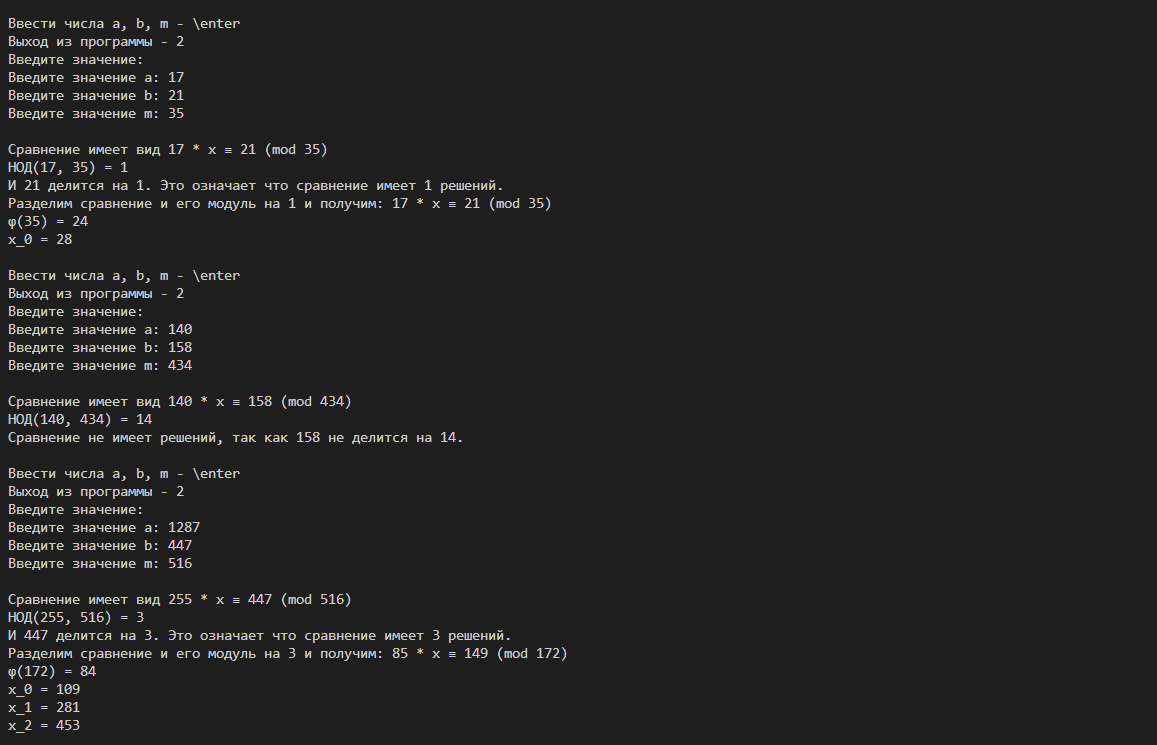
\includegraphics[width=0.8\textwidth]{pic1.png}
    \caption{}
\end{figure}

\setminted[python]{linenos,breaklines=true, fontsize=\small, style=bw}
    \subsection{Код программы, реализующей рассмотренный алгоритм}
        \inputminted{python}{lab2.py}

\end{document}